\chapter{Reinforcement-Learned Balancing}
\label{chap:rl_walk}

\section{Introduction}

A major goal of the RoboCup Standard Platform League is the development of improved bipedal control of the Nao robots. The teams aim to demonstrate that the robots are able to execute increasingly human-like bipedal behaviours, whether it be walking, kicking a ball, or self-stabilisation. The ability to execute these types of movements, to be able to switch between them fluidly, and to react against external forces to avoid falling over is a key research area in robotics. The responsiveness required by such movements is what is to be expected of future robots particularly when emulating human behaviours, as in playing a game of soccer.

Such behaviour is extremely difficult or practically impossible to be programmed directly into a robot. Careful study and analysis of human movement is required and mathematical models must be derived to approximate it. Even then, such models tend only to work in ideal situations, such as walking over a perfectly smooth and flat ground. In order to approach the behaviour that is inherent in humans -- that of adapting to any possible situation -- it is necessary that machine-learning principles are considered in order to adapt to any change in the robot's environment. For example, a hand-programmed walk will react differently over a rough and bumpy surface than over a flat and smooth surface, as it is confined to a small subset of possible robot states, whereas a machine-learned walk should in theory be able to react to either.

For the 2013 Open Challenge, we explored the application of Reinforcement-Learned behaviours for bipedal movements on the Nao robots. We aimed to demonstrate that simulator-learned behaviours could be applied directly to the Nao robots without the need for significant tuning in software. The Open Challenge entry was titled \textit{``Stability Control through Machine Learned Behaviours''}\cite{openchallenge}.

The learned behaviours aimed to react to a greater number of states than hand-programming would allow for and to allow relatively simpler implementation of more advanced behaviours. Applied to the Naos, we aimed for self-stabilisation without the need for hard-coding in a variety of states including: changing support feet at different frequencies (walking on the spot); standing upright; standing on either foot; and seamlessly switching between these. 

\newpage
\section{Background \& Related Work}

Reinforcement Learning (RL) is a method of deriving software models for behaviour through machine learning. RL is used to automatically determine a model for actions to be taken given an ``environment state'' such that the maximum ``reward'' can be achieved. In the context of stability control for bipedal robots, RL results in a software model (known as a \textit{policy}) which states what motors the robot should actuate and in what manner, given that the robot is in some state (the environment state) and wants to reach some position (the reward).

An RL model is defined by:\cite{bernhard_rl}

\begin{description}
\item[States] -- the set of all states the robot can be expected to act in.
\item[Actions] -- the set of all actions the robot can potentially take.
\item[Transitions] -- the definition of how states transition into other states.
\item[Reward] -- the definition of how good being in a certain state or doing a certain action is.
\end{description}

%The Q-learning -> learns to assign values to (s,a) pairs.
%Given a particular action in a particular state, followed by actions which follow a particular policy, the agent will receive a particular set of reinforcement.

RL works by finding a function which gives the value of taking a particular action when in a particular state and then following the optimal policy thereafter. The optimal value is therefore the best one of the possible actions that can be taken at a given state. The ``value'' of each state-action is dependent on the reward -- taking actions which lead to rewards quickly is of higher value, taking actions which lead to slow or negative rewards is of lower value.

The work presented in this report relies primarily on the application of RL research done by Hengst\cite{bernhard_rl}. Hengst's work involved the use of a simulated environment for the robot, allowing for fast reinforcement learning of optimal policies for various behaviours (defined by their cost (inverse of reward) functions), including:

\begin{itemize}
\item Standing upright and still.
\item Standing on one leg.
\item Rocking between both legs.
\end{itemize}

Hengst's work allows for a much simpler implementation of the policies in real hardware with less need for learning or tuning on the hardware. Testing this is one of the primary aims of the work outlined in this report.

White's\cite{white} 2011 implementation of a simulator-learned policy for a walking gait on the Naos is also an important motivator. White was able to show that a simulator-learned walk running on the Naos was able to react to obstacles significantly better than one with no RL policy. However, White also found that state measurement was very difficult due to noisy sensors and limited data, and the work was not merged into the competition code.

Further work by Liu\cite{liu} in 2012 focused primarily on improving state measurement by introducing heavy filtering of the Inertial Measurement Unit (IMU) located in the chest of the Naos. While the demonstrated filters worked well, Liu found that the underlying assumptions in the filter (that the robot is standing still, upright, and approximates an inverted pendulum) were not sufficient when introducing more complex motion such as a walking gait.

\section{Theory \& Implementation}

\subsection{Learning the Control Policies}
In learning the policies for the behaviours, Hengst\cite{bernhard_rl} defines a robot model, including as much accuracy in the links, joints, masses, etc. as possible -- an example of this is seen in Figure~\ref{fig:lean}.

\begin{figure}[h]
\centering
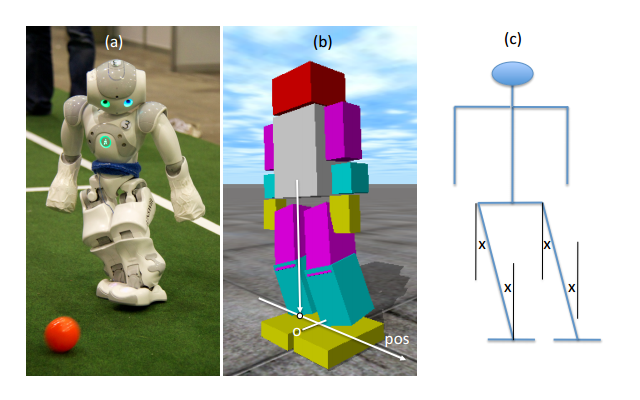
\includegraphics[width=3.5in]{img/RL_lean.png}
\caption{The Nao robots modelled as a $23 DOF$ (Degree of Freedom) system in (b). \cite{bernhard_rl}}
\label{fig:lean}
\end{figure}

Hengst defines the \textit{state} of the robot using two variables:
\begin{itemize}
\item position of the middle of the torso in $m$eters
\item velocity of the middle of the torso in $\sfrac{m}{s}$
\end{itemize}

The goal or reward function of a behaviour is therefore based on getting to some state (as in standing still) or reaching some states at a certain time (as in rocking back and forth). Example policies can be seen in Figure~\ref{fig:policy_diagram}.

\begin{figure}[!h]
\centering
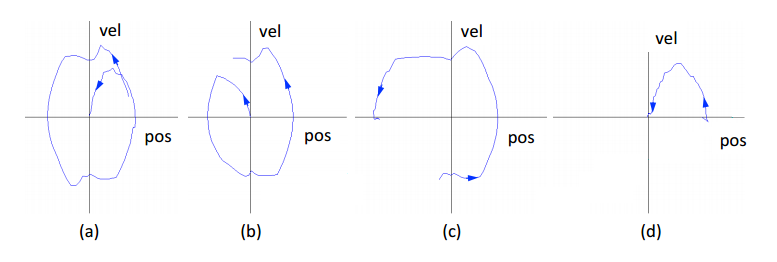
\includegraphics[width=5in]{img/RL_policies.png}
\caption{Example of learned policies in the two state variables (position and velocity). The policy defines what actions to take which will lead to the state approaching some goal (for example, zero position and velocity for standing still, as in (a)).\cite{bernhard_rl}}
\label{fig:policy_diagram}
\end{figure}

Knowing how the state of the environment changes based on actions is what the transition function defines. The transition function is calculated by observing the change between states of the simulation when subjected to a random choice of actions (from the set of actions that could be taken) -- the random simulation essentially explores the state space of the model through the actions. This is a computing-intensive process (taking upwards of several hours to complete, depending on the desired resolution) but is also practically impossible to define through real-life hardware testing (due to the complexity in analysing the environment, something a simulation can do very easily).

Once the state transitions are known (to whatever degree), it is a simple case of calculating the value of each state-action for any given reward function, and then finding the optimal action to take for a given state-action (that is to say, the action to take depends not only on the current state, but also on the previous action taken). The list of optimal actions for each state-action is then known as the \textit{optimal policy}. A reward function can be easily created for any goal desired, such as standing still or walking on the spot, so long as the goal states are in the set of explored states. Knowing the state transitions also allows for quick switching between behaviours by simply picking which policy to follow.

A total of 7 goal states were defined: 6 in the coronal plane (side-to-side motions), and 1 in the sagittal plane (front-to-back motions). These goals were as follows:

\begin{enumerate}
\item Standing still
\item Fast pace rocking between feet
\item Medium pace rocking between feet
\item Slow pace rocking between feet
\item Standing on right leg
\item Standing on left leg
\item Sagittal: standing still
\end{enumerate}

The optimal policy for these goals is given as a simple output of numbers, simply being the state-action pair and the corresponding optimal action to take. An example output from a control policy can be seen in Figure~\ref{fig:policy}.

The reinforcement learning then learns the actions required for optimal stabilisation of given behaviours, as well as for the transition between behaviours. These actions are used in the creation of policies, which define the action required for each possible state of the robot. Some simplified example policies can be seen in Figure \ref{fig:policy_diagram}.


\begin{figure}[h]
\newcommand\statehighlight[1]{\textcolor[rgb]{1,0,0}{#1}}
\newcommand\actionhighlight[1]{\textcolor[rgb]{0,0,1}{#1}}
\begin{Verbatim}[commandchars=\\\{\},frame=single]
// Policy table for 6 Coronal behaviours
// State-action is defined by: Goal, lateral torso position, 
//                             lateral torso velocity, 
//                             last action taken
// Action: 0 for ankle roll left, 1 for no action, 
//         2 for ankle roll right
//  \statehighlight{state-action}    \actionhighlight{action}
   0 -0.08 -0.4  0     0
   0 -0.08 -0.39 0     1
   0 -0.08 -0.38 0     1
   0 -0.08 -0.37 0     2
\end{Verbatim}
\caption{An excerpt of a control policy for coronal behaviours.}
\label{fig:policy}
\end{figure}

\subsection{State Measurement}

The Nao robots contain an Inertial Measurement Unit (IMU) in their chest, consisting of 2 gyrometers and a three-axis accelerometer.\cite{nao_imu} By knowing the location of the IMU, most importantly its height from the bottom of the feet (dimensions given by Aldebaran Robotics), and ensuring this matches with the simulator, one can use simple trigonometry to calculate the required position and velocity state variables. 

As seen in Figure~\ref{fig:trig}, we can define a simple axis system from the IMU, with the $x$-axis pointing towards the front of the robot, the $y$-axis towards the side, and the $z$-axis pointing down to the ground. This coordinate system also applies to the three-axis accelerometer, which provides a $\sfrac{m}{s^2}$ acceleration reading for each of these axes. This can be used to help calibrate the gyrometer readings, as the accelerometer should expect to read $9.81\sfrac{m}{s^2}$ for the $z$-axis and $0\sfrac{m}{s^2}$ for the $x$- and $y$-axes when the robot is standing upright and still.

% TODO fig:trig

The position and velocity of the IMU is taken with respect to its neutral position, when the robot is standing upright. In this way, it is expected that the coronal (side to side) position of the IMU is exactly centered between the two feet. The two gyrometers provide an angular measurement of the torso, being the angle of lean about the $x$-axis (the coronal ``roll'') and the lean about the $y$-axis (the sagittal ``pitch''), as seen in Figure~\ref{fig:trig}. When standing upright the torso is expected to be at a pitch angle of $0\degree$ relative to the hip pitch (which depends on the way the legs are bent while in a standing position), and a roll angle of $0\degree$.

Now, if we assume small perturbations to the torso (in other words, only small pitch and roll angles will be in the state space of the policy), then we can approximate the position of the torso by simply using the gyrometer measurements and the known height of the IMU from the base of the feet. As seen in Figure~\ref{fig:triangle}, we have an isosceles triangle (with two equal sides being the height of the IMU) and the angle between them is known. We can easily calculate the horizontal displacement of the IMU by with $pos = H * \sin{\theta}$. Furthermore, for small angles of $|\theta| < 20\degree$, we know that $\sin{\theta} \approx \theta$ (in radians). Thus, we can approximate the lateral position of the IMU by simply multiplying the lean measurement by some constant close to the known height.

\begin{figure}[h]
\centering
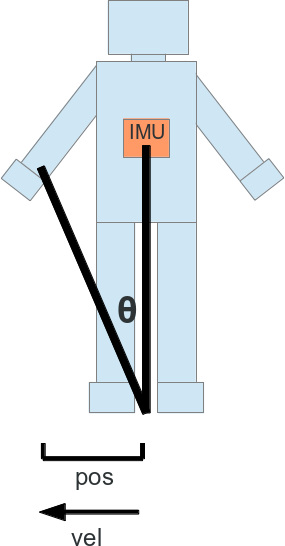
\includegraphics[width=1.5in]{img/lean_trig.png}
\caption{The coronal state variables are the lateral position and velocity of the IMU in the torso of the Nao robots.}
\label{fig:triangle}
\end{figure}

Work was done on state measurement by Liu\cite{liu} through extensive filtering of the IMU's measurements.

\subsection{Policy Implementation}

The work done in this year was an attempt to combine the previous works of Hengst, White, and Liu in order to produce these self-stabilising behaviours, and to explore the application to walk stabilisation.

% TODO: Talk about generic policy file

Much of the work done is in fact an incremental improvement to White's policy implementation, as well as the application of the improved policies done by Hengst.


The policy tables are then interpreted by the real-world Nao robots, allowing them to mimic the behaviour seen in the simulation by actuating joints to follow the optimal action sequence.

\section{Results}
%TODO \section{Evaluation}

The three-axis accelerometer was found to be too noisy to be of any significant use. While standing still, the accelerometer would report a large acceleration reading in the $z$-axis (as expected due to gravity), but also non-zero and wildly fluctuating accelerations in the $x$- and $y$-axes. Heavy filtering of these was found to be ineffective, as the offset from zero tended to drift randomly.



Overall results of the policy implementation were mixed. Sagittal self-balancing control when standing still was found to be a significant improvement over no control policy. Upon being disturbed, the robot would actuate its hip motors and oscillate its body back into an upright position. This was objectively more effective method than when the robot's stiff body was simply allowed to rock back and forth with no use of the controller, as the test results show below.

% TODO Table of test results


Despite disappointing behaviour in the field, the presentation of the work was considered worthy of $3^{rd}$ place in the Open Challenge.


\section{Future Work}

% TODO More complex state measurement

\section{Conclusions}
